

\begin{figure}[h!]
\centering
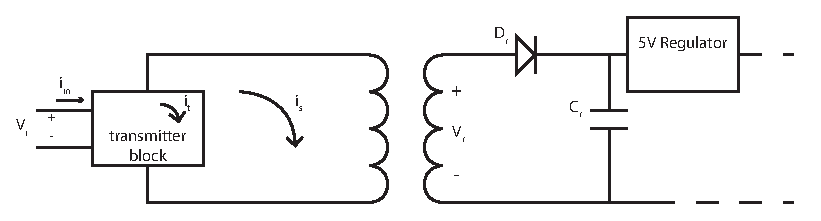
\includegraphics[width=1\textwidth]{design.pdf}
\caption{Internet of things chain of actions}
\label{fig:design1}
\end{figure}

 split the figure into charge cycle and discharge cycle
The Figure \ref{fig:design1}
shows a low level schematic of the receiver and charging circuit which will be the main focus of our project. The induction current $i_r$ induced by the transmitter through magnetic coupling will be the main source of charging current. The current $i_c$ charges the super capacitor $C_s$ up to the capacity of $V_c$, in our case $V_c \leq 5$ Volts the maximum voltage rating of super capacitor, $i_b$ charges the battery and $i_L$ is consumed by the current limiting resistor $R_L$  and a light source $LED$. Where $i_r = i_c + i_b +i_L$ . Now in analysis lets first consider the efficiency ${\eta}$ of the circuit.
If $P_{o}$ is the power consumed by the receiver and $P_{i}$ is the power provided by the transmitter, ignoring small power drops across $D_r$ and $C_r$  then:
\begin{equation}\label{eq:effb}
 {\eta} = \frac{P_o}{P_i}
\end{equation}
where $P_o = V_{reg} \times i_r $ and $P_i = V_i \times i_s $
The battery at receiving end when fully charged can provide $V_l = 3 $ Volts.
For 3 Volts lithium-ion battery the output voltage normally drops by $0.2 $ Volts when battery is at $40 \%$ of its capacity and can go to $2.6 $ Volts when almost drained \cite{IAmp}. Hence a slight dim in LED brightness can be observed as battery drains with time.
% \cite{IAmp}. http://www.ibt-power.com/Battery_packs/Li_Ion/Lithium_ion_tech.html
For normal brightness of $LED$ with forward voltage drop of $V_{drop} = 1.7 $ Volts we choose $i_L = 20 $ mA then using equation ~\ref{eq:load} we found $R_L = 65 \Omega $
\begin{equation}\label{eq:load}
 R_L = \frac{V_l - V_{drop}}{i_L}
\end{equation}
To find out with what power ratings of $R_L$ should be used we can use $P_L = {i_L}^2 \times R_L $ which gives us $P_L = 400 \mu$ Watts, which is the power dissipated at $R_L$ and can be avoided if we use a LED that has exactly the same forward voltage drop $V_{drop}$ as the battery output $V_l$ that will remove the need of $R_L$. However, LED is very sensitive to even small change in the applied voltage, a voltage change of 0.1 Volt can cause the LED current $i_L$ to shot up beyond the limits hence a more careful consideration is required if one chooses to omit the current limiting resistor $R_L$.
%\subsection{Battery Life}
The battery that we are using has a capacity of 50 mAh, which means if current $I_B$ of 50 mA  is continuously drawn from the battery then it can last for one hour. To find out total battery life for our circuit we need to consider the total power consumed $P_c$, for our case $P_c = i_L \times V_l $ from which we can calculate total life of fully charged battery.

 $Total Battery Life = \frac{Battery Capacity}{Power Consumed}$
                    $= \frac{I_B \times V_l \times 1 hour}{i_L \times V_l}$
                    $= \frac{50mA \times 3V \times 1 hour}{20mA \times 3V}$
                    $= 2.5 hours$


%\subsection{Charging Profile}
Now lets consider how the charging and discharging of the receiver circuit works. According to manufacturer specification $i_r \leq 400 $ mA , which enforces the limit for the system to function properly.
In figure %~\ref{fig:rec_design}
the super capacitor $C_s$ has very low series resistance of $0.07 \Omega$ compared to $R_L = 65 \Omega$ hence during charging we can say that $i_c \approx i_r$ and if the $i_r(t)$ is not constant and depends on time then the capacitor charging is governed by the following equation
\begin{equation}\label{eq:cap}
 V_c = V_{reg} \left(1 - e^{\frac{-t}{R_cC}}\right)
\end{equation}
where $R_c$ is the series limiting resistance of receiver circuit whose value depends on the maximum value of $i_r$ and $C$ is the total capacitance of super capacitor which in our case $C_s = 5 $ Farads
$R_c$ can be chosen using $R_c = \frac { V_{reg}}{i_r} $ for maximum allowed $i_r = 400$ mA which gives us $R_c = 12.5 \Omega$

\begin{figure}[h!]
\centering
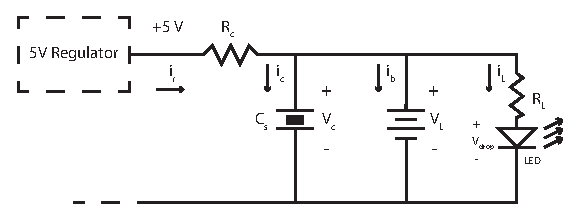
\includegraphics[width=1\textwidth]{rec_design.pdf}
\caption{Internet of things chain of actions}
\label{fig:rec_des}
\end{figure}


Figure \ref{fig:rec_des}
shows charging, discharging and idle profile of the super capacitor during the system operation. In initial charging cycle $t_{ci}$, $C_s$ is charged using $i_r(t)$ following equation \ref{eq:cap} and during discharge cycle $t_d$, the $i_r(t) = 0$ and discharge current is supplied in the form of $i_b$ and $i_L$. Finally during the equilibrium cycle $t_{eq}$ the voltage is reduced to equal the battery voltage ($V_l = 3$ V) such that no current flows between the battery and super capacitor and $i_b = 0$, at this stage only battery's charge is used to power the LED. At last during the second charge cycle $t_{c2}$, the capacitor's charging starts from equilibrium voltage instead of 0 and is charged to $V_{reg}$ un till the discharge cycle starts again.
